\subsection{Applications}
\begin{frame}{}
    \LARGE Autoencoders: \textbf{Applications}
\end{frame}

\begin{frame}{Autoencoders: Applications}
    \centering
    \large{\textbf{Applications of Autoencoders}}
    \begin{itemize}
        \item Dimensionality Reduction
        \item Super-Resolution
        \item Colorization
        \item Anomaly Detection
        \item Denoising
    \end{itemize}
\end{frame}

\begin{frame}[allowframebreaks]{Dimensionality Reduction}

Autoencoders help us reduce the number of features in our data, similar to PCA, but in a more flexible way.

\begin{itemize}
    \item The encoder takes big, complex data and squeezes it into a smaller, simpler form.
    \item This smaller version keeps the important information.
    \item Great for making it easier to see patterns or to prepare data for other machine learning tasks.
\end{itemize}

\textbf{Example}: We can use autoencoders to turn images (like MNIST digits) into just 2 or 3 numbers, so we can plot and explore them easily.

\framebreak

\begin{figure}
    \centering
    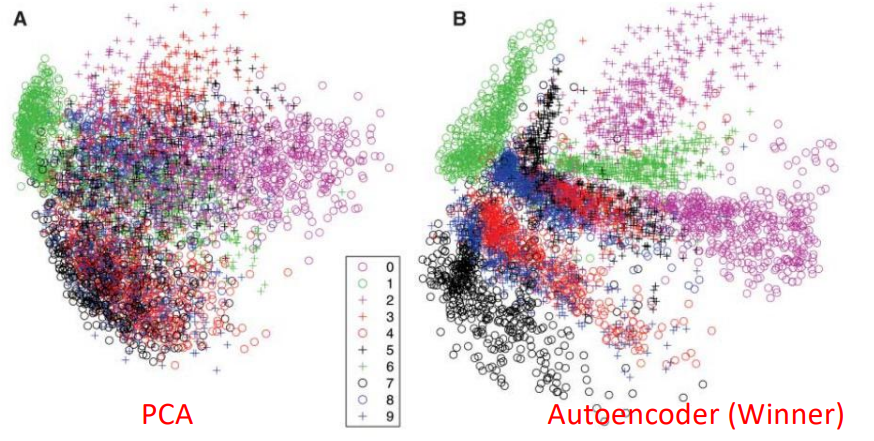
\includegraphics[height=0.75\textheight, width=\textwidth, keepaspectratio]{images/autoencoders/image_representation.PNG}
    \caption*{t-SNE visualization on MNIST digits dataset. PCA vs. Autoencoders. The image vector is projected into $\mathbb{R}^2$.}
\end{figure}

\end{frame}
\begin{frame}[allowframebreaks]{Super-Resolution}

Autoencoders can be used to reconstruct high-resolution images from their low-resolution counterparts.

\begin{itemize}
    \item Input: Low-resolution image.
    \item Output: High-resolution image.
    \item Often implemented with convolutional layers for spatial pattern learning.
\end{itemize}
\textbf{Use Case}: Enhancing medical images, satellite images, or upscaling low-resolution photos.

\framebreak

\begin{figure}
    \centering
    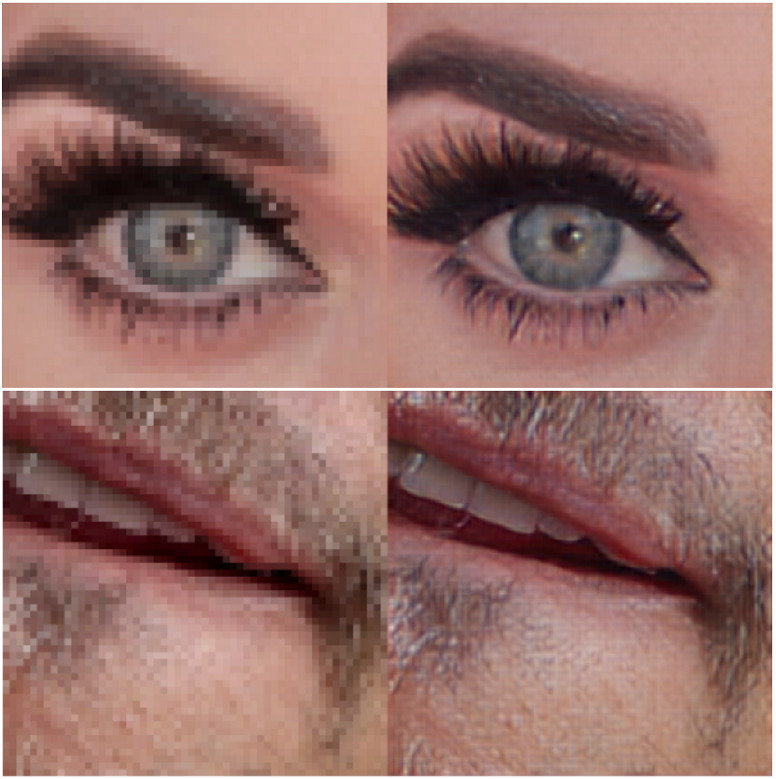
\includegraphics[height=0.8\textheight, width=\textwidth, keepaspectratio]{./images/autoencoders/image_enhancement.png}
    \caption*{Image super-resolution using Autoencoders}
\end{figure}

\end{frame}
\begin{frame}[allowframebreaks]{Image Colorization}

Autoencoders can learn to predict color information for grayscale images.

\begin{itemize}
    \item Input: Grayscale image (1 channel).
    \item Output: Colorized image (3 channels — RGB).
    \item Requires learning semantic and contextual relationships to apply realistic colors.
\end{itemize}

\textbf{Use Case}: Restoring historical black-and-white photos.

\framebreak

\begin{figure}
    \centering
    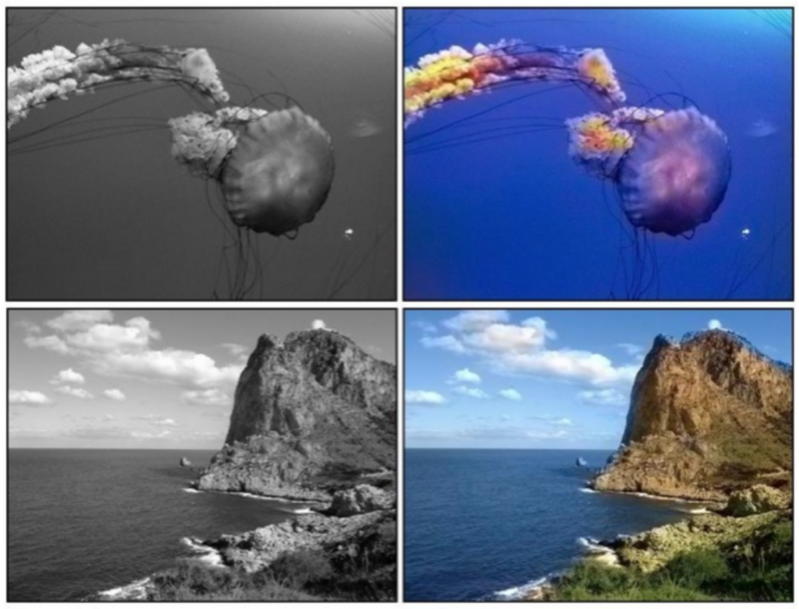
\includegraphics[height=0.8\textheight, width=\textwidth, keepaspectratio]{./images/autoencoders/image_colorization.png}
    \caption{Image colorization using Autoencoders}
\end{figure}

\end{frame}
\begin{frame}[allowframebreaks]{Anomaly Detection}
    \begin{itemize}
        \item Autoencoders are trained to reconstruct input data.
        \item During training, the model learns to compress and decompress data that is similar to the training set (normal data).
        \item When presented with anomalous (outlier) data, the reconstruction error increases, as the autoencoder cannot effectively reconstruct unseen patterns.
    \end{itemize}

    \textbf{Use Cases:}
    \begin{itemize}
        \item Fraud detection in financial transactions
        \item Fault detection in industrial systems
        \item Intrusion detection in cybersecurity
        \item Medical anomaly detection (e.g., rare diseases in imaging)
    \end{itemize}

    \framebreak
    \begin{figure}
        \centering
        \fetchconvertimage{https://www.mdpi.com/IoT/IoT-04-00016/article_deploy/html/images/IoT-04-00016-g002.png}{images/autoencoders/anomaly-detection.png}{width=0.8\textwidth,keepaspectratio}
        \caption*{Structure of the deep autoencoder (AE) for anomaly detection and feature extraction for multi-classification of cyber-attacks.}
    \end{figure}

    \framebreak
    \begin{figure}
        \centering
        \fetchconvertimage{https://www.researchgate.net/profile/Huaiqiang-Sun/publication/367509994/figure/fig1/AS:11431281115469461@1674921049910/Overview-of-the-proposed-autoencoder-based-anomaly-detection-framework-A-Training-the.png}{images/autoencoders/anomaly-detection-brain.png}{height=0.68\textheight,keepaspectratio}
        \caption*{Autoencoder-based anomaly detection framework: A) Training the autoencoder for modeling the distribution of healthy brain anatomy. B) In the inference phase, anomaly maps reveal lesions by subtracting their reconstruction from the input image. C and D) Details of the proposed autoencoder.}
    \end{figure}
    
\end{frame}
\section{Denoising}
\begin{frame}{}
    \LARGE Diffusion Models: \textbf{Denoising}
\end{frame}

\begin{frame}[allowframebreaks]{Denoising Diffusion Probabilistic Models}
    
Denoising diffusion models, also known as score-based generative models, have recently emerged as a powerful class of generative models. They achieve remarkable results in high-fidelity image generation, often outperforming GANs.
\begin{figure}
    \centering
    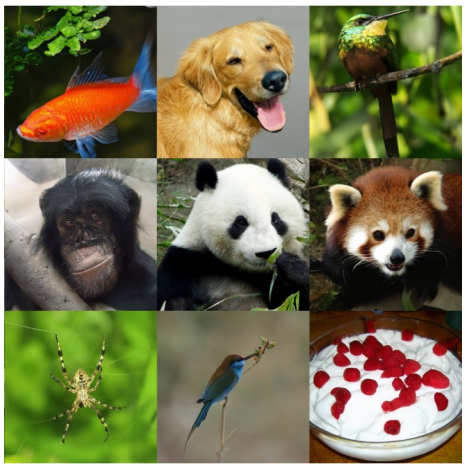
\includegraphics[height=0.5\textheight, width=\textwidth, keepaspectratio]{images/diffusion/diff_results_1.png}
    \caption*{Diffusion Models Beat GANs on Image Synthesis \href{https://arxiv.org/abs/2105.05233}{Dhariwal \& Nichol, OpenAI, 2021}}
\end{figure}

\framebreak
Denoising diffusion models consist of two processes:
\begin{itemize}
    \item A fixed (predefined) \textbf{forward diffusion process} $q$, which gradually adds Gaussian noise to an image until only pure noise remains.
    \item A learned \textbf{reverse denoising diffusion process} $p_\theta$, where a neural network is trained to gradually denoise an image starting from pure noise, eventually recovering the original image.
\end{itemize}

\begin{figure}
    \centering
    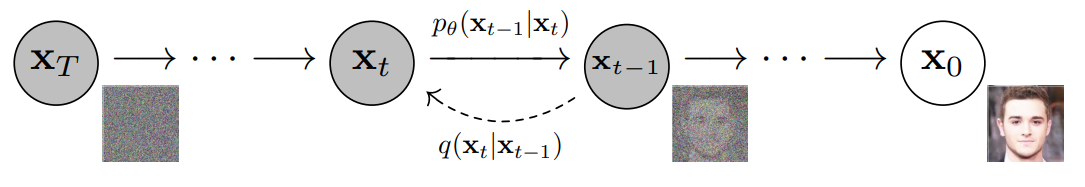
\includegraphics[height=0.8\textheight, width=\textwidth, keepaspectratio]{images/diffusion/diff_3.png}
\end{figure}

\framebreak

\begin{figure}
    \centering
    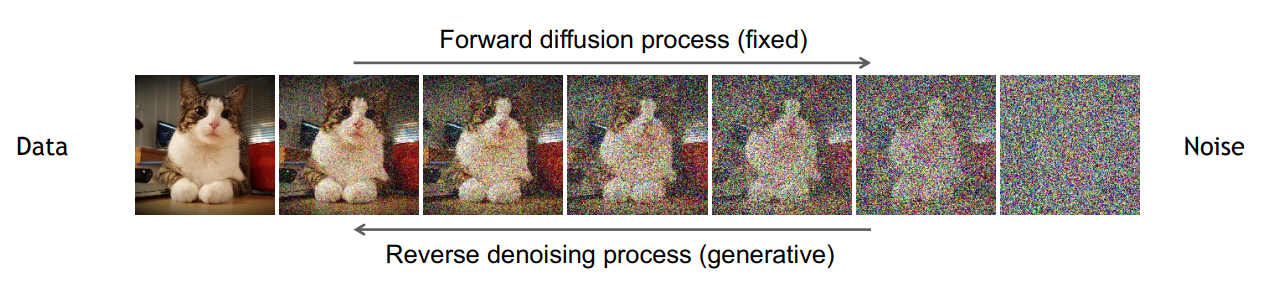
\includegraphics[height=0.9\textheight, width=\textwidth, keepaspectratio]{images/diffusion/diffusion_1.png}
\end{figure}

\end{frame}

% \begin{frame}[allowframebreaks]{Autoencoders: Applications}
% \textbf{Dimensionality Reduction}

% Autoencoders are widely used as nonlinear alternatives to traditional dimensionality reduction techniques like PCA (Principal Component Analysis).
% \begin{itemize}
%     \item The encoder compresses high-dimensional data into a low-dimensional latent space.
%     \item This latent representation preserves meaningful features and patterns.
%     \item Especially effective for visualizing data or preprocessing inputs for downstream tasks.
% \end{itemize}
% \textbf{Use Case}: Visualizing high-dimensional datasets (e.g., MNIST) in 2D or 3D.

% \framebreak

% \begin{figure}
%     \centering
%     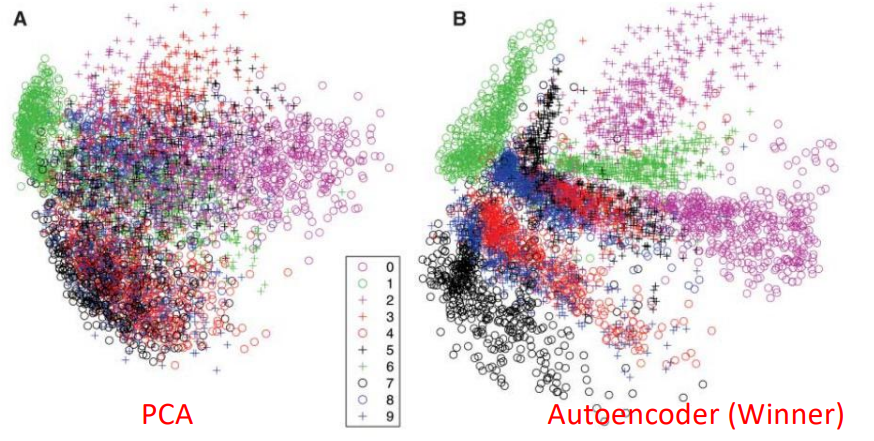
\includegraphics[height=0.8\textheight, width=\textwidth, keepaspectratio]{images/autoencoders/image_representation.PNG}
%     \caption{t-SNE visualization on MNIST digits dataset. PCA vs. Autoencoders. The image vector is projected into $\mathbb{R}^2$.}
% \end{figure}

% \framebreak

% \textbf{Super-Resolution}

% Autoencoders can be used to reconstruct high-resolution images from their low-resolution counterparts.

% \begin{itemize}
%     \item Input: Low-resolution image.
%     \item Output: High-resolution image.
%     \item Often implemented with convolutional layers for spatial pattern learning.
% \end{itemize}
% \textbf{Use Case}: Enhancing medical images, satellite images, or upscaling low-resolution photos.

% \framebreak

% \begin{figure}
%     \centering
%     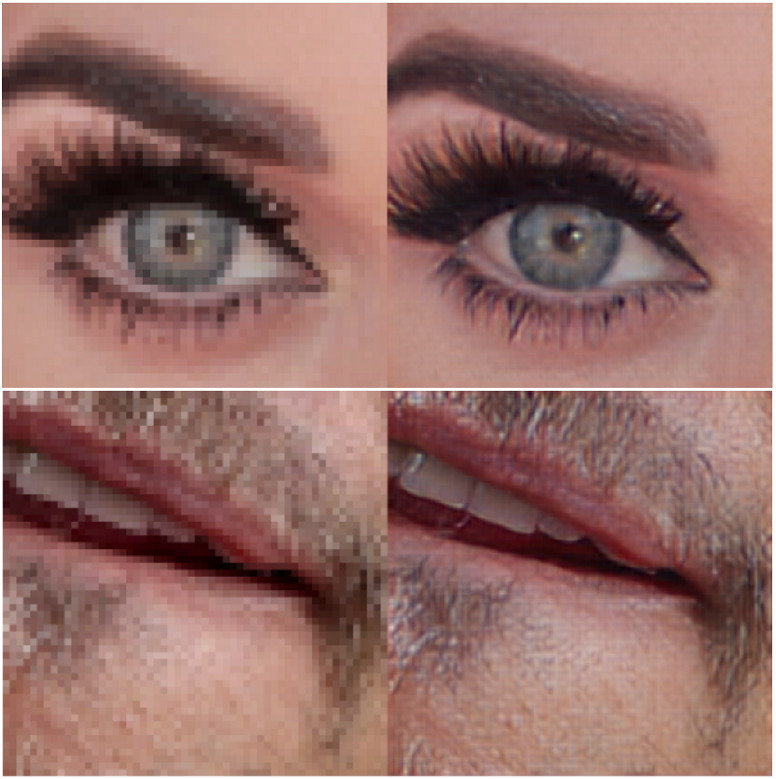
\includegraphics[height=0.8\textheight, width=\textwidth, keepaspectratio]{./images/autoencoders/image_enhancement.png}
%     \caption{Image super-resolution using Autoencoders}
% \end{figure}

% \framebreak

% \textbf{Image Colorization}

% Autoencoders can learn to predict color information for grayscale images.

% \begin{itemize}
%     \item Input: Grayscale image (1 channel).
%     \item Output: Colorized image (3 channels — RGB).
%     \item Requires learning semantic and contextual relationships to apply realistic colors.
% \end{itemize}
% \textbf{Use Case}: Restoring historical black-and-white photos.

% \framebreak

% \begin{figure}
%     \centering
%     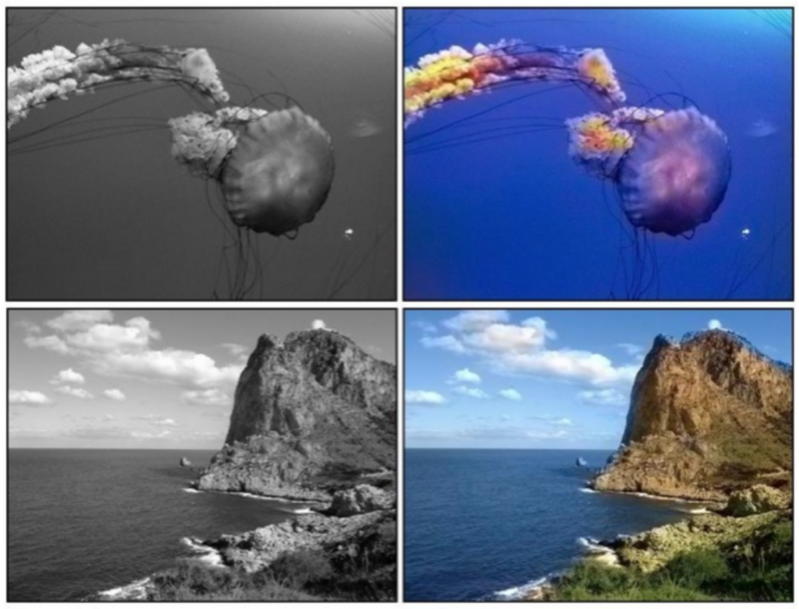
\includegraphics[height=0.8\textheight, width=\textwidth, keepaspectratio]{./images/autoencoders/image_colorization.png}
%     \caption{Image colorization using Autoencoders}
% \end{figure}

% \end{frame}
